\section{Methodology}
\label{sec-methodology}

%Describe your approach and design
%Instead of simply explaining what you ended up doing, show why you made such
%design decisions / how what the trade-offs are.

As mentioned earlier, DRAM power consumption is dominated by
charging/discharging chip capacitances and signal reflections caused by link
terminations. Once the capacitors have reached steady state, their power
consumption is negligible in comparison to the system as a whole and thus can
be neglected from our power models. Instead we focus on link termination and
signal reflections. Specifically, DDR4 memory technology leverages \TT{DBI} to
reduce the signal reflections and power consumption. Intuitively, DBI aims to
reduce the number of bit flips (DBI-AC) and binary signal probabilities
(DBI-DC) to improve power consumption of read and write operations. For
reducing bit flips, take for example the case where memory location $M$
previously had the value $00000000$ that was being overwritten by the value
$11111111$. Instead of flipping every bit in $M$, a DBI-AC enabled memory system
would retain the previous state of $00000000$ and set the DBI flag that
signifies that all the bits are flipped.  This would incur the power consumption
of 1 bit flip, not the entire data byte.  Since the power consumption of 0 and
1 is not the same, depending on memory technology constraints, DBI-DC aims to
reduce the prevalence of the higher power consuming bit. In the case of DDR4,
$0$ consumes more power and thus DBI aims to reduce the number of $0$'s and
increase the number of $1$'s \fixme{add citation}. Figure \ref{fig:dbi-dc}
illustrates the impact of DBI-DC on improving signal quality and consequently
power consumption of read and write operations. The larger open data eye
illustrates that there is less interference between the driver and reflected
signals when using DBI-DC and the smaller $V_{pp}$ suggests that the driver has
to work less with DBI-DC enabled.

\begin{figure}[!htb]
  \centering
  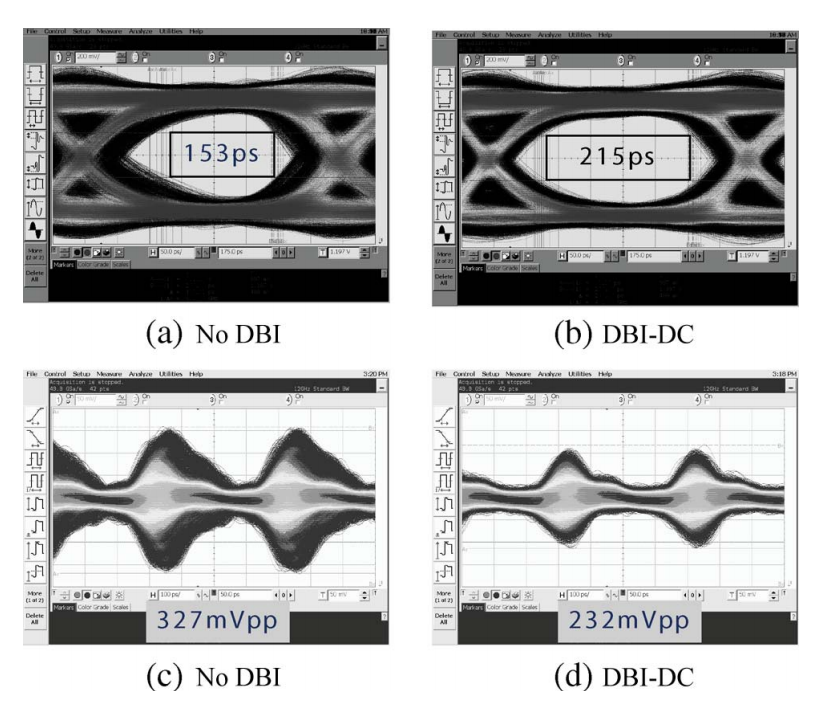
\includegraphics[width=0.3\textwidth]{figs/dbi-dc}
  \caption{Using DBI-DC increases the open data eye and reduces the required
  $V_{pp}$ for effectively driving the DRAM chip. Taken from \cite{hollis}}
  \label{fig:dbi-dc}
\end{figure}

The following sections outline our model, and experimental setup for measuring
the ODT power overhead of memory encryption on DBI-enabled DDR4 memory
technology.

\subsection{Model}
In order to model the power overhead of memory encryption on DBI-enabled memory
technologies, we use the same model described by Hollis \cite{hollis}, shown
below:

    $$ P_t = A \times P_{dc} + B \times P_{ac}$$

Where $P_t$ is the ODT power consumption, $P_{dc}$ is the intrinsic DC-power
consumed and $P_{ac}$ is the intrinsic AC-power consumed by bit flips. The
ratios $A$ and $B$ determine the DC and AC factors of $P_t$ respectively.
DBI-DC aims to exploit program structure and reduce $A$ whereas DBI-AC aims to
reduce $B$. Together they can significantly decrease the ODT power consumption.
As Hollis \cite{hollis} describes - under the assumption that data written to
memory or read from memory are completely random:

  $$ A = 0.5$$
  $$ B = 0.5$$

Intuitively, truly random data would have equal probability of each binary
digit making $A = 0.5$. Similarly, truly random data would have equal
probability of flipping or not flipping and thus, $B = 0.5$. In order to model
ODT power consumption, we must determine the values of $A$ and $B$ for secure
memory systems with encryption and insecure memory systems without encryption.
The following sections outline our experimental setup for analyzing the DBI
enabled power model described.

\subsection{Experimental Setup}

\begin{figure}[!htb]
  \centering
  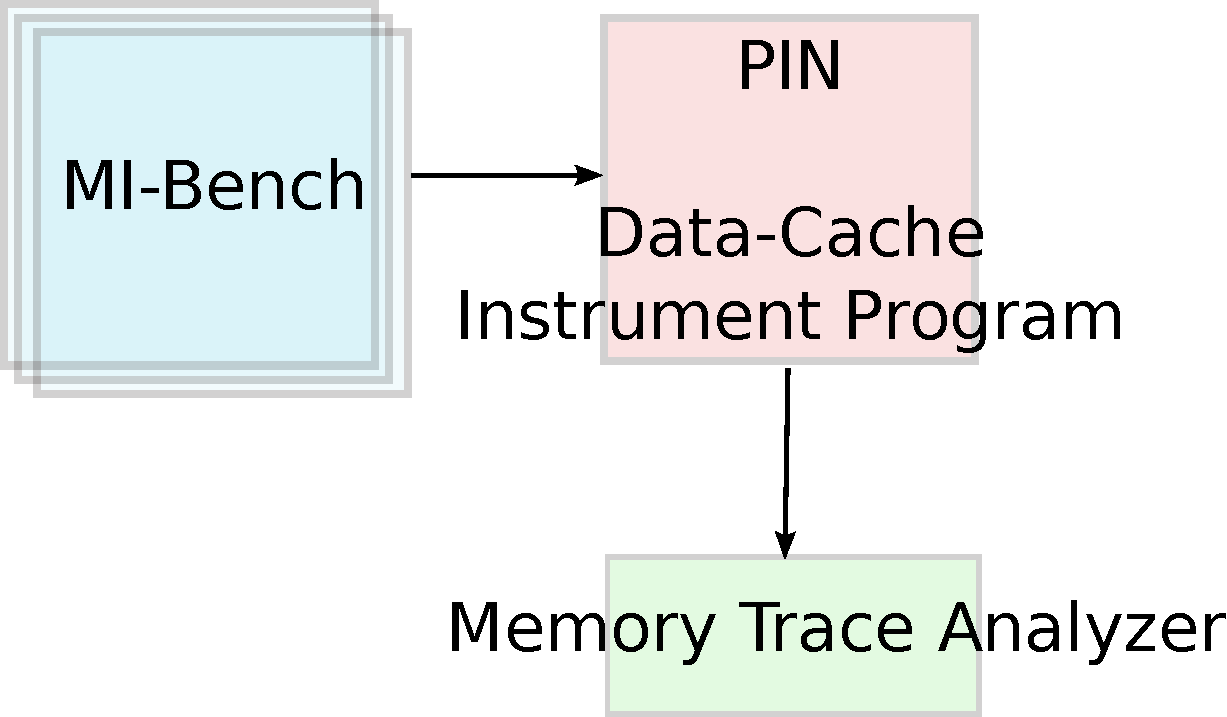
\includegraphics[width=0.3\textwidth]{figs/exp-design}
  \caption{General system architecture for the experimental setup for analyzing
  the DBI enabled power model}
  \label{fig:exp}
\end{figure}

Figure \ref{fig:exp} illustrates the general experimental setup we used to
implement the DBI model described earlier. First, we need a set of
representative benchmarks to run through to generate realistic memory traces
that can be used to analyze the effect of memory encryption on power
consumption. We chose MiBench \cite{mibench} for our benchmark suite. MiBench
consists of applications representative of embedded and mobile workloads and
provides easy to use build binary executables which integrates well with the
\TT{PIN} architectural simulator we used. We chose not to use the \TT{SPEC2006}
benchmark as the applications targeted workloads handled by general purpose
processors. We used 28 applications in the MiBench suite (the following 14
applications on big and small data-sets):

\begin{multicols}{2}
  \centering
  \begin{enumerate}
    \item \TT{basicmath}
    \item \TT{bitcount}
    \item \TT{qsort}
    \item \TT{susan}
    \item \TT{jpeg}
    \item \TT{dijkstra}
    \item \TT{patricia}
    \item \TT{stringsearch}
    \item \TT{blowfish}
    \item \TT{sha}
    \item \TT{adpcm}
    \item \TT{CRC32}
    \item \TT{FFT}
    \item \TT{gsm}
  \end{enumerate}
\end{multicols}

The chosen set of MiBench applications spans all six classes provided by the
benchmark: \TT{automotive}, \TT{consumer}, \TT{network}, \TT{office},
\TT{security}, and \TT{telecomm}.

\subsubsection{Architectural Simulator}
In order to analyze the impact of memory encryption on DBI-enabled DDR4 memory
systems, we need to generate memory traces from the MiBench applications.
Traditional simulator such as \TT{Gem5} \cite{gem5} and \TT{ESESC} \cite{esesc}
did not meet our constraints. Gem5 and ESESC for the purposes of this study
required significant overhead in terms of establishing an environment and
integrating the simulators with MiBench applications to generate usable memory
traces. Instead we chose use \TT{Pin} \cite{pin} - a dynamic binary
instrumentation tool developed by Intel as a lean, easy to use computer
architectural simulator. Since Pin performs run-time program instrumentation
analysis on compiled binary files, integrating Pin with MiBench required little
effort. Once we generated the specific \TT{Pintool} to generate memory traces,
we could simply run the Pin simulator providing the Pintool and compiled
Mibench application binaries as inputs.

Leveraging the IA-32 instruction set architecture framework provided by Pin, we
created a \TT{Pintool}, to output the memory trace of arbitrary compiled
binaries. That is, we used the \TT{dcache} and \TT{safecopy} examples provided
to create a single Pintool that provided a trace of all first-level cache
misses. On every miss, the Pintool would output whether the operation was a
\TT{load} or \TT{store} operation, the address and the value being read or
written to memory. Unlike Gem5 and ESESC, Pin does not provide a cycle-by-cycle
timing trace for when specific architectural events occur. Though this may be
efficient for system-wide power analysis, our model is not parametrized on time
but only the specific bit values of data units being read and written. In our
experience, Pin worked well for generating such a coarse, event based memory
trace.

For the purposes of our study we only simulated the data-cache with : 32KB
total size, 8-way associativity, and 128B cache line size. The Pintool we
generated allows the user to input a defined size, associativity and line size.
The specific parameters chosen were used in previous Pin exercises as the
default configuration and seemed reasonable for our study.

\begin{enumerate}
  \item PIN - dynamic binary instrumentaiton tool : describe cache settings
  \item DRAMSim - Did not work for us.
  \item Python Script to analyze the loads and stores from the trace outptted
    from PIN
\end{enumerate}
